\documentclass[10pt, letterpaper]{article}
\usepackage[utf8]{inputenc}
\usepackage[margin=1.25in]{geometry}
\usepackage{times}
\usepackage{natbib}
\usepackage{hyperref}
\usepackage{amsmath}
\usepackage{amssymb}
\usepackage{graphicx}
\usepackage{booktabs}
\usepackage{lipsum} % for dummy text

% Handle Unicode characters from bibtex
\usepackage{newunicodechar}
\newunicodechar{τ}{$\tau$}
\newunicodechar{♫}{}

% Mock formatting to resemble an ICLR submission
\usepackage{titlesec}
\titleformat{\section}{\large\bfseries}{\thesection}{1em}{}
\titleformat{\subsection}{\normalsize\bfseries}{\thesubsection}{1em}{}

\title{\vspace{-1cm}\Large \bf PUT YOUR SEARCH WHERE YOUR DOUBT IS: THE BEHAVIORAL BRITTLENESS OF LLMS IN EXTERNAL TOOL USAGE}

\author{
  \textbf{Dvir Lafer} \\
  Technion - Israel Institute of Technology \\
  \and
  \textbf{Omer Nahum} \\
  Technion - Israel Institute of Technology \\
  \and
  \textbf{Eyal Ben-David} \\
  Google \\
  \and
  \textbf{Jonathan Herzig} \\
  Google \\
  \and
  \textbf{Eran Ofek} \\
  Google \\
  \and
  \textbf{Idan Szpektor} \\
  Google \\
  \and
  \textbf{Roi Reichart} \\
  Technion - Israel Institute of Technology \\
  \and
}
\date{}

\newcommand{\doi}[1]{doi: \href{https://doi.org/#1}{\nolinkurl{#1}}}

\begin{document}
\maketitle

\begin{abstract}
While existing benchmarks for Large Language Models (LLMs) predominantly emphasize performance metrics such as accuracy, the evaluation of agentic systems necessitates assessing the generalization of their \emph{behavior}. In this work, we investigate behavioral generalization within a multi-hop information-seeking framework. Our analysis reveals a critical gap: although LLMs are aligned to aggressively invoke search tools when encountering uncertainty on standard benchmark questions, this learned behavior fails to generalize, degrading significantly when these queries are paraphrased into naturalistic user prompts with identical information needs. We demonstrate that this mis-generalization can be mitigated by optimizing uncertainty alignment during post-training via on-policy rollouts. These findings highlight the importance of distinguishing a model's tool-use alignment from its raw uncertainty, providing a foundation for future research into the behavioral failure modes of agentic LLMs to ensure reliable tool usage and mitigate the spread of misinformation.
\end{abstract}

\section{Introduction}

The widespread adoption of Large Language Models (LLMs) has catalyzed a paradigm shift from traditional tools to autonomous agents across various domains, such as conversational systems, finance, and complex information-seeking workflows \cite{abbasian_conversational_2024, xiao_tradingagents_2025}. In particular, systems designed for ``deep research'' now routinely automate rigorous multi-step research by integrating LLMs with advanced information retrieval and autonomous reasoning \cite{xu_comprehensive_2025}. As \citet{xu_comprehensive_2025} highlight in their comprehensive survey, while these systems demonstrate significant capabilities, they also present profound ethical and technical challenges regarding information accuracy and reasoning control. As users increasingly offload manual research to AI in an era rampant with misinformation, ensuring the reliability of these agents is paramount.

To be reliable, it is not enough for models to perform well on highly structured multi-hop training datasets. They must develop a generalized behavioral policy for info-seeking that functions robustly across diverse, real-world interactions. A robust model should consistently recognize its knowledge gaps (epistemic uncertainty) and invoke tools appropriately, regardless of how a user phrases their query. However, our core observation reveals a critical failure: \textbf{the mis-generalization of agentic behaviors}. While models may appear to learn tool-use policies (via SFT or RL) that yield high accuracy on benchmark templates \cite{chu_self-critique_2025}, these learned behaviors often act as overfitted heuristics. When real-world users formulate naturalistic queries that deviate from benchmark priors, the agents' behavior severely degrades.

Existing evaluation paradigms often mask this mis-generalization. A substantial body of work addresses LLM uncertainty to mitigate intrinsic hallucinations \cite{yona_can_2024, manakul_selfcheckgpt_2023, kuhn_semantic_2023, liu_metafaith_2025}, and explores the general efficacy of tool usage \cite{bai_qwen_2023, lu_toolsandbox_2025, keren_matter_2026, barres_2-bench_2025, ning_wtu-eval_2024} or the interplay between parametric knowledge and external context \cite{cheng_understanding_2024, yang_crag_2024, li_understanding_2024}. Yet, they predominantly measure performance metrics on structured datasets like HotpotQA \cite{yang_hotpotqa_2018} and MusiQue \cite{trivedi__2022}. Preliminary findings suggest brittleness to prompt variations \cite{jang_how_2026, rabinovich_robustness_2025}, but the extent to which agents fail to generalize their info-seeking behavior—specifically the active process of composing search queries based on their own uncertainty—remains largely overlooked.

In this work, we put this behavioral mis-generalization at the center of our investigation. Using the MusiQue benchmark as a foundation, we introduce a mechanism to evaluate how tool-use policies shift when transitioning from standard benchmark phrasings to naturalistic user queries that share the exact same information need. Our extensive analysis confirms a severe behavioral brittleness: while LLMs already struggle with uncertainty gaps on standard queries, their agentic behavior—measured by search efficiency, hop-level uncertainty alignment, and premature commitment to answers—breaks down significantly under natural paraphrasing.

Finally, we demonstrate that this mis-generalization can be mitigated. We perform an intervention by training a LoRA adapter for Nemotron-3-nano using on-policy rollouts, proving that a quantifiable uncertainty alignment signal exists and can be explicitly targeted during post-training. By disentangling a model's raw capabilities from its behavioral alignment, we aim to spotlight critical failure modes in modern LLMs and inspire further research into robust, generalized agentic systems that resist the spread of misinformation.

\section{Related Works}

\textbf{Agentic Information-Seeking and Tool Evaluation} -- Existing evaluations of tool-augmented LLMs predominantly focus on downstream performance metrics, such as final answer accuracy \cite{wei_browsecomp_nodate, cheng_facts_2025, trivedi__2022}. However, end-to-end evaluations often mask the behavioral policies driving the agent, such as the necessity, efficiency, and correctness of individual search queries. Uncalibrated tool usage can harm agents by either bloating the context window or fetching irrelevant results that distract the model from its correct parametric knowledge. While recent benchmarks \cite{ning_wtu-eval_2024, lu_toolsandbox_2025} assess the overall necessity of tool calls, they largely lack the resolution to evaluate multi-step, per-hop search behavior. To decouple model capabilities from specific search engines \cite{cheng_facts_2025}, our setup uses an external search API, allowing us to systematically evaluate the efficiency of search trajectories, including sequential redundancy and missed knowledge hops.

\textbf{Uncertainty Estimation and Knowing When to Search} -- A prerequisite for autonomous information-seeking is the model's ability to recognize its own knowledge gaps---its epistemic uncertainty. Extensive research has focused on estimating uncertainty to mitigate intrinsic hallucinations \cite{yona_can_2024, raj_measuring_2023, farquhar_detecting_2024}, with semantic entropy emerging as a reliable metric. However, less attention has been given to whether this internal uncertainty correctly triggers actionable agentic behavior, such as issuing a search query. In this work, we utilize semantic entropy as a ground-truth measure of epistemic uncertainty, enabling us to directly quantify the calibration between a model's knowledge gaps and its active search behavior.

\textbf{Behavioral Brittleness and Mis-generalization} -- As agents are deployed in real-world applications, their robustness to naturalistic user interactions is paramount. Recent findings have surfaced the issue of prompt brittleness in agentic workflows, demonstrating that models are highly sensitive to instructional variations \cite{jang_how_2026, rabinovich_robustness_2025}. Our work extends these findings by quantifying the behavioral mis-generalization of info-seeking agents. We show that while models may appear calibrated on standard benchmark templates, their behavior degrades significantly under natural paraphrasing---exhibiting premature answer commitment and uncalibrated search queries. Crucially, we demonstrate that this uncertainty alignment can be recovered and explicitly targeted during post-training.
\section{Research Questions}
To structure our analysis, we propose the following research questions:
\begin{itemize}
    \item \textbf{RQ1:} Do models behave differently on benchmark questions vs. real users' questions?
    \item \textbf{RQ2:} Are models' search calls aligned with their epistemic (per-hop) uncertainty?
    \item \textbf{RQ3:} Are models' search calls efficient (right volume, right hops)?
    \item \textbf{RQ4:} Does verbalized commitment to an answer change with phrasing?
\end{itemize}

\section{Experimental Setup}

\subsection{Datasets}
Our primary substrate for evaluation is a staleness-filtered slice of 600 multi-hop questions from the MusiQue \citep{trivedi__2022} validation set, retained because each carries a gold \emph{hop decomposition}. To facilitate post-training intervention via SFT, we also filtered approximately 1,000 questions from the MusiQue training set to generate on-policy rollouts. Furthermore, to evaluate generalization to real users, we manually curated 101 information-seeking questions from the ShareChat and WildChat datasets.

\subsection{On-Policy Rollouts}
To create training data for our SFT intervention, we ran Nemotron-3-nano with access to a search tool over the natural paraphrases and analyzed the traces online. We retained only the traces that contained queries fulfilling all uncertain hops, and strictly removed any traces with queries attributed to certain hops.

\subsection{The Hop-Level Diagnostic Instrument}\label{sec:setup}

We instantiate our study on three production-grade agentic systems---\textbf{Gemini~3.1
Pro}, \textbf{Qwen~3.5 (122B)}, and \textbf{Nemotron Nano (30B)}---using a shared web-search tool to isolate behavioral differences. 

To separate model behavioral shifts from mere difficulty variations, we utilize a single \emph{hop-level
diagnostic protocol}. For each question $q$ with gold hops
$\{h_j\}$ we (1)~sample the agent five times in closed-book mode and compute a per-hop
\textbf{semantic entropy} $\mathcal{E}_j$ \citep{farquhar_detecting_2024, kuhn_semantic_2023}; a hop is \emph{uncertain}
if $\mathcal{E}_j>0$ and \emph{certain} otherwise. We then (2)~run the agent on the full
question with search enabled, and (3)~use an LLM judge to attribute
every emitted search query to a specific hop $j$. The cross-product of uncertainty and search partitions \emph{every per-hop decision}
into interpretable cells, analogous to a binary classification taxonomy: \textbf{Effective (E)} (True Positive: uncertain hop, searched), \textbf{Correct Parametric (CP)} (True Negative: certain hop, not searched), \textbf{Parametrically Redundant (PR)} (False Positive: certain hop, searched anyway), and \textbf{Missed (M)} (False Negative: uncertain hop, not searched).
The closed-book uncertainty $\mathcal{E}_j$ is a property of the underlying
fact and is reused across phrasings, ensuring any movement between cells reflects a change in
\emph{behavior}, not in difficulty.

\subsection{Constructing User-Like Queries}\label{sec:paraphrase}

The benchmark surface form leaks the retrieval strategy by exposing the
hop chain through nested relative clauses and a named bridge entity. A real user with the
same information need would instead ask something like ``\emph{I'm curious about Bill
Cockcroft's background---what region did he study in?}'' To produce such queries at scale
while holding the information need fixed, we rewrite the $600$ questions under verifiable constraints (no intermediate bridge entity, no relative-clause pattern).
We call this first rewrite set \textbf{MuSiQue-Natural} (Natural~1).

To control for potential confounding factors like leaked bridge entities or drifted information needs, we generate a second, audited rewrite set,
\textbf{MuSiQue-Natural2} (Natural~2), using a \emph{generate$\to$judge$\to$regenerate}
validation loop. A rewrite is accepted only if it leaks no bridge entity and
is judged strictly equivalent to the original. Natural~2 serves as a \emph{conservative} condition to verify that our findings are a genuine response to user-like surface forms. The same loop is reused
to paraphrase 101 real user queries from the ShareChat dataset for generalization checking.

\begin{table}[ht]
  \centering
  \small
  \begin{tabular}{p{0.15\linewidth} p{0.25\linewidth} p{0.25\linewidth} p{0.25\linewidth}}
    \toprule
    \textbf{Dataset} & \textbf{Formal / Benchmark} & \textbf{Natural 1 / Real User} & \textbf{Natural 2} \\
    \midrule
    \textbf{MusiQue} & What was the name of the spouse of the first convert to the most prevalent religion in Jordan? & I've been wondering about the early history of the dominant religion in Jordan. Could you tell me who the spouse of the first convert to that faith was? & I'm interested in the early history of Jordan's main faith. Who was the wife of the very first person to convert to it? \\
    \midrule
    \textbf{ShareChat} & Which country lost its entire national territory after its military chose war to reclaim lost land instead of conceding peace? & ``Can you name any times in history where a military had the chance to concede peace, but chose war to reclaim lost territory and ended up losing the entire country?'' & \textit{N/A} \\
    \bottomrule
  \end{tabular}
  \caption{Concrete examples of query paraphrasing from MusiQue and ShareChat, demonstrating the transition from formal benchmark structures (e.g., nested relative clauses) to naturalistic user queries.}
  \label{tab:paraphrase_examples}
\end{table}

\section{Results}

\begin{figure}[t]
  \centering
  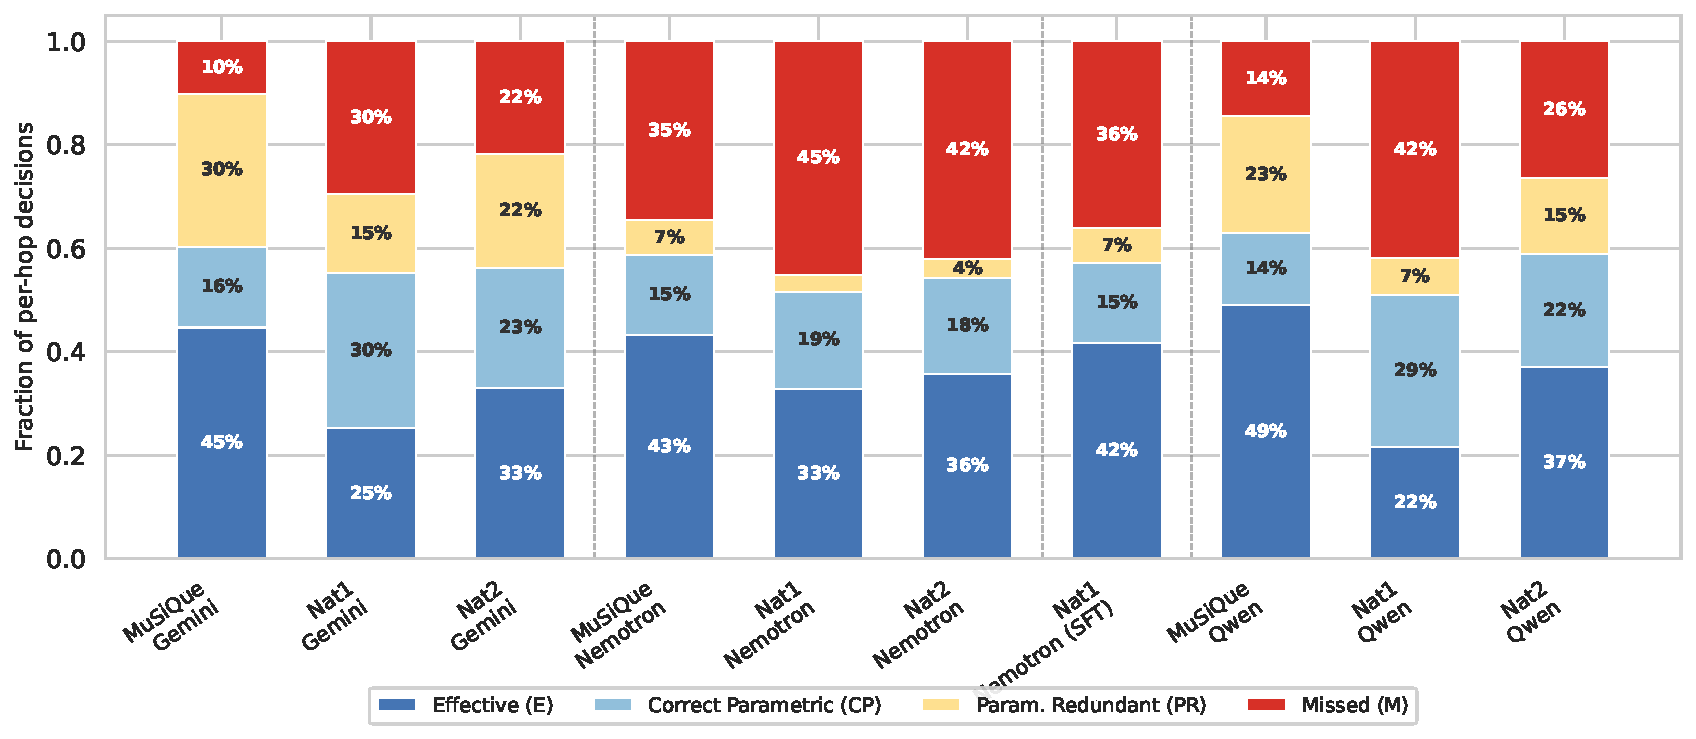
\includegraphics[width=\linewidth]{Figures/fig1_quadrant_taxonomy_simple.pdf}
  \caption{Per-hop decision taxonomy (Effective, Correct Parametric, Parametrically Redundant, and Missed) for each model under formal, Natural~1, and Natural~2 phrasing. Across all three models, user-like rewrites contract the Effective (True Positive) cell and expand the Missed (False Negative) cell, demonstrating severe uncertainty misalignment.}
  \label{fig:taxonomy}
\end{figure}

\begin{figure}[t]
  \centering
  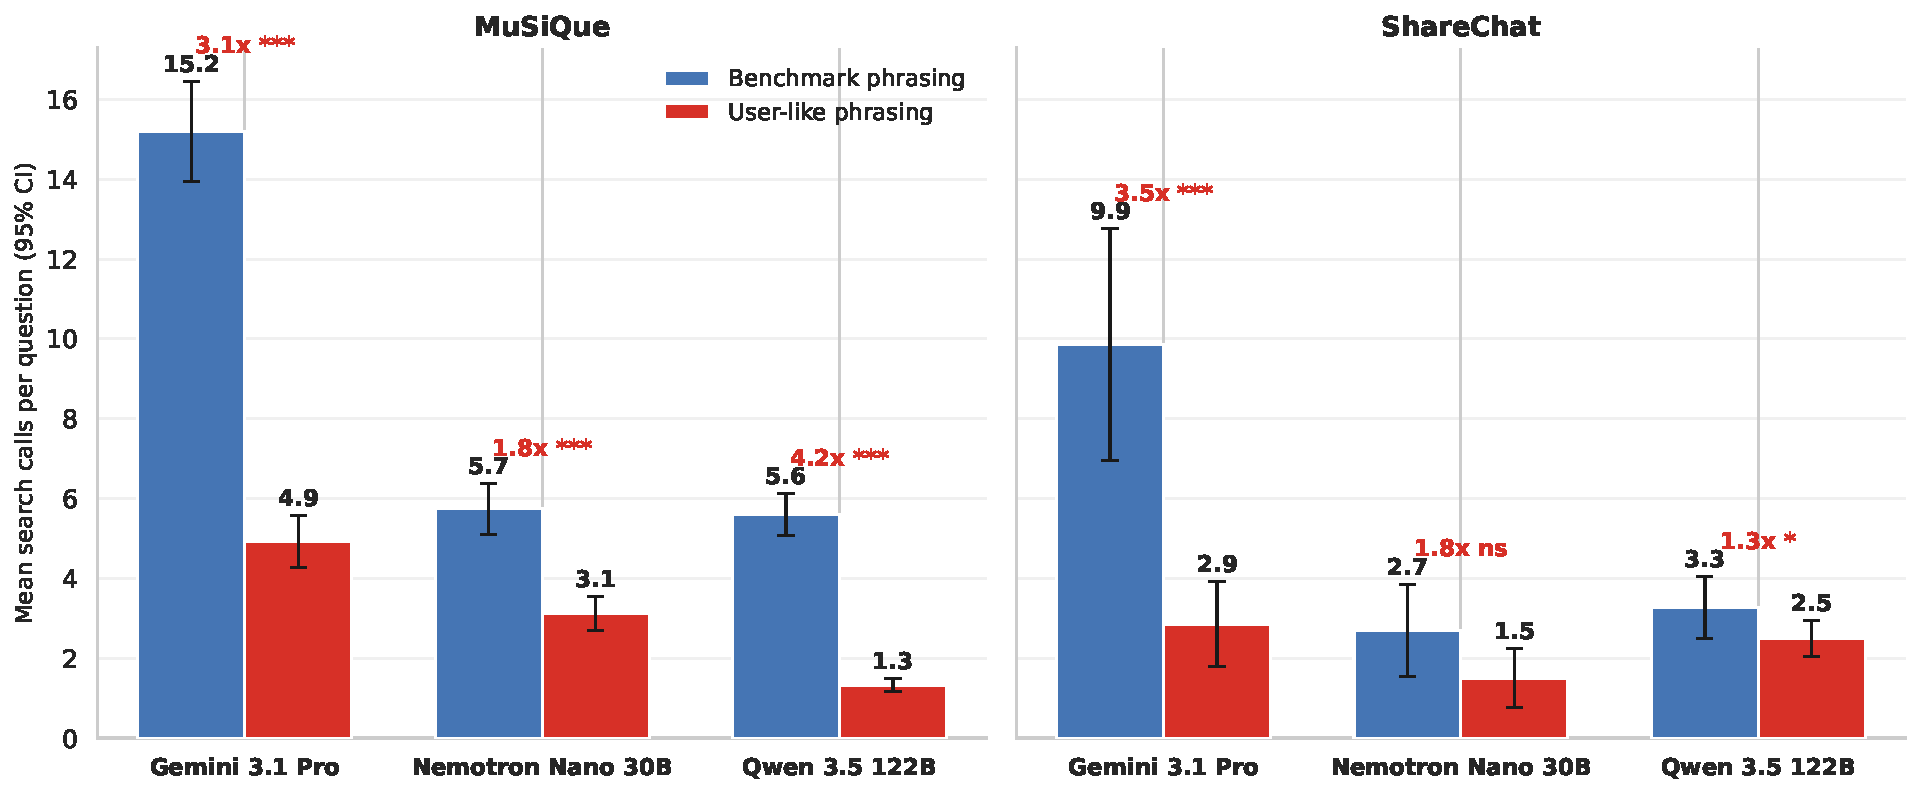
\includegraphics[width=0.8\linewidth]{Figures/sharechat_search_comparison.pdf}
  \caption{Average number of search queries per question. A sharp collapse in search volume is observed when transitioning from formal benchmark-style paraphrases to real user queries from ShareChat.}
  \label{fig:sharechat}
\end{figure}

\subsection{Search Collapse and Uncertainty Misalignment}\label{sec:collapse}

Our primary finding is that agentic search policies fail to generalize from benchmark phrasing to naturalistic user queries. Mean searches per question drop sharply (by 46--76\%, with a 65\% pooled drop) from the formal benchmark to Natural~1, and the gap survives the audited paraphrase (Natural~2), confirming it is not a rewriting artifact. Furthermore, this effect generalizes to real user queries: evaluating 101 real information-seeking queries from ShareChat shows a similar search volume collapse of 24--71\% (57\% pooled) relative to their formal benchmark-style paraphrases (Figure~\ref{fig:sharechat}).

\begin{figure}[t]
  \centering
  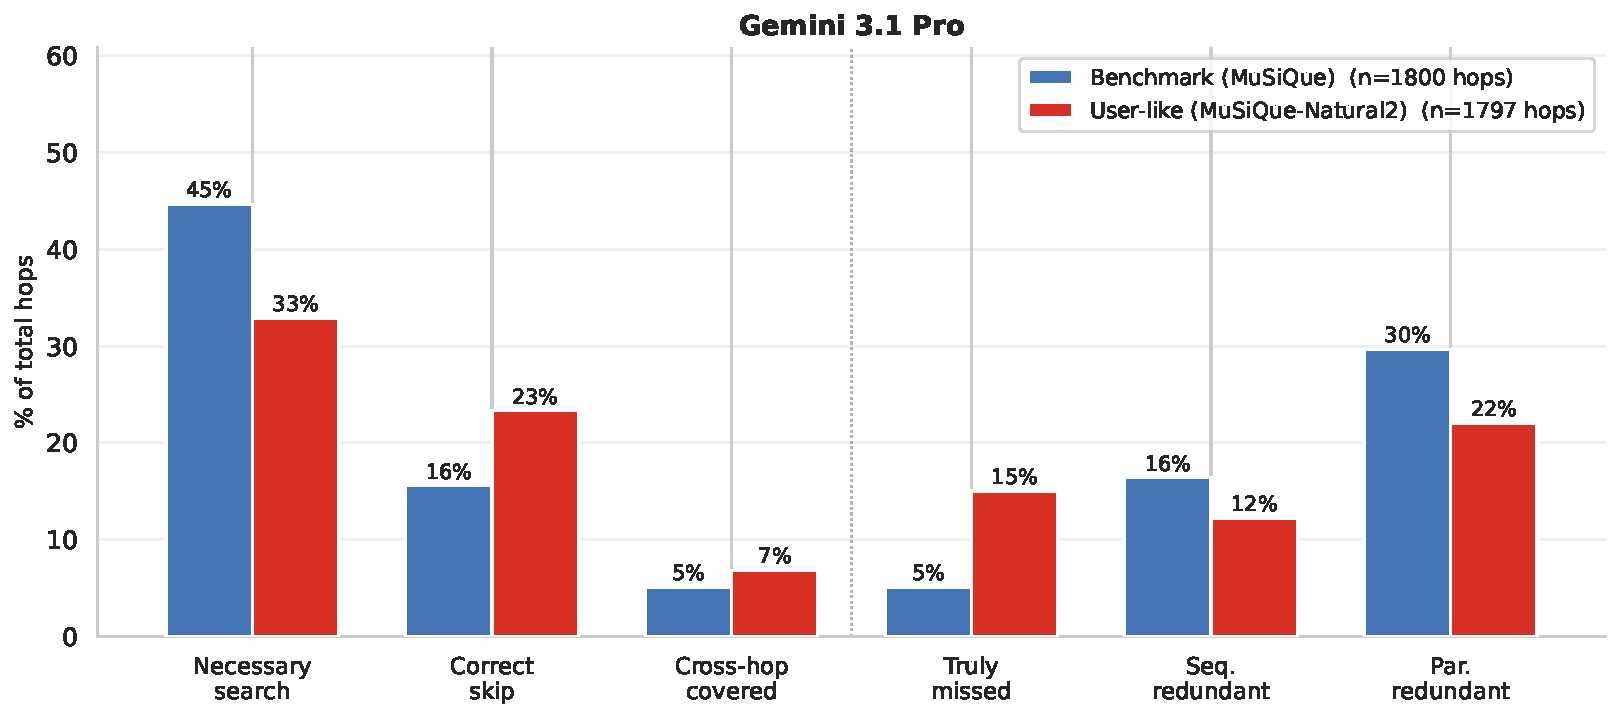
\includegraphics[width=0.8\linewidth]{Figures/search_calibration_extended_gemini_3_pro_preview.pdf}
  \caption{Search calibration for Gemini 3.1 Pro. The plots contrast the model's search behavior against its epistemic uncertainty. The shift from formal to user-like phrasing triggers a massive increase in missed necessary searches.}
  \label{fig:calibration}
\end{figure}

Crucially, the searches that survive are heavily misaligned with the model's epistemic uncertainty. The dominant cell-level movement under the rewrite is $E\!\to\!M$: the agent stops searching precisely the hops it had flagged as uncertain. The \emph{Missed} cell grows significantly by +11 to +27 percentage points across all models, with the \emph{Effective} cell contracting by a matching amount (Figure~\ref{fig:taxonomy}). This severe breakdown in calibration is further detailed in Figure~\ref{fig:calibration}.

\textbf{The Accuracy Disconnect.} While behavioral degradation is stark, end-task aggregate accuracy remains flat. We attribute this disconnect to several noise confounders inherent to end-to-end evaluations, which mask true agentic capabilities: (1) \textbf{Parametric Leakage:} models may have been exposed to the MusiQue dataset during training; (2) \textbf{Uncertainty Spectrum:} uncertainty is continuous rather than binary. Recent work demonstrates that computing uncertainty at the level of meaning---by marginalizing over semantic equivalences---provides a principled, continuous measure of an LLM's epistemic uncertainty \citep{kuhn_semantic_2023}, which robustly detects hallucinations where simple likelihoods fail \citep{farquhar_detecting_2024}. Consequently, a ``missed'' search might involve a fact the model could partially recall, allowing it to guess correctly without searching (Appendix~\ref{app:knowledge_tiers}); and (3) \textbf{Noisy Web Search:} the reduction in search volume under natural phrasing inadvertently acts as a regularization mechanism against retrieving distracting context. Because end-to-end accuracy is heavily confounded by these factors, it masks the underlying breakdown in agentic behavior, underscoring why our hop-level diagnostic is necessary to evaluate tool-use alignment.



\begin{figure}[t]
  \centering
  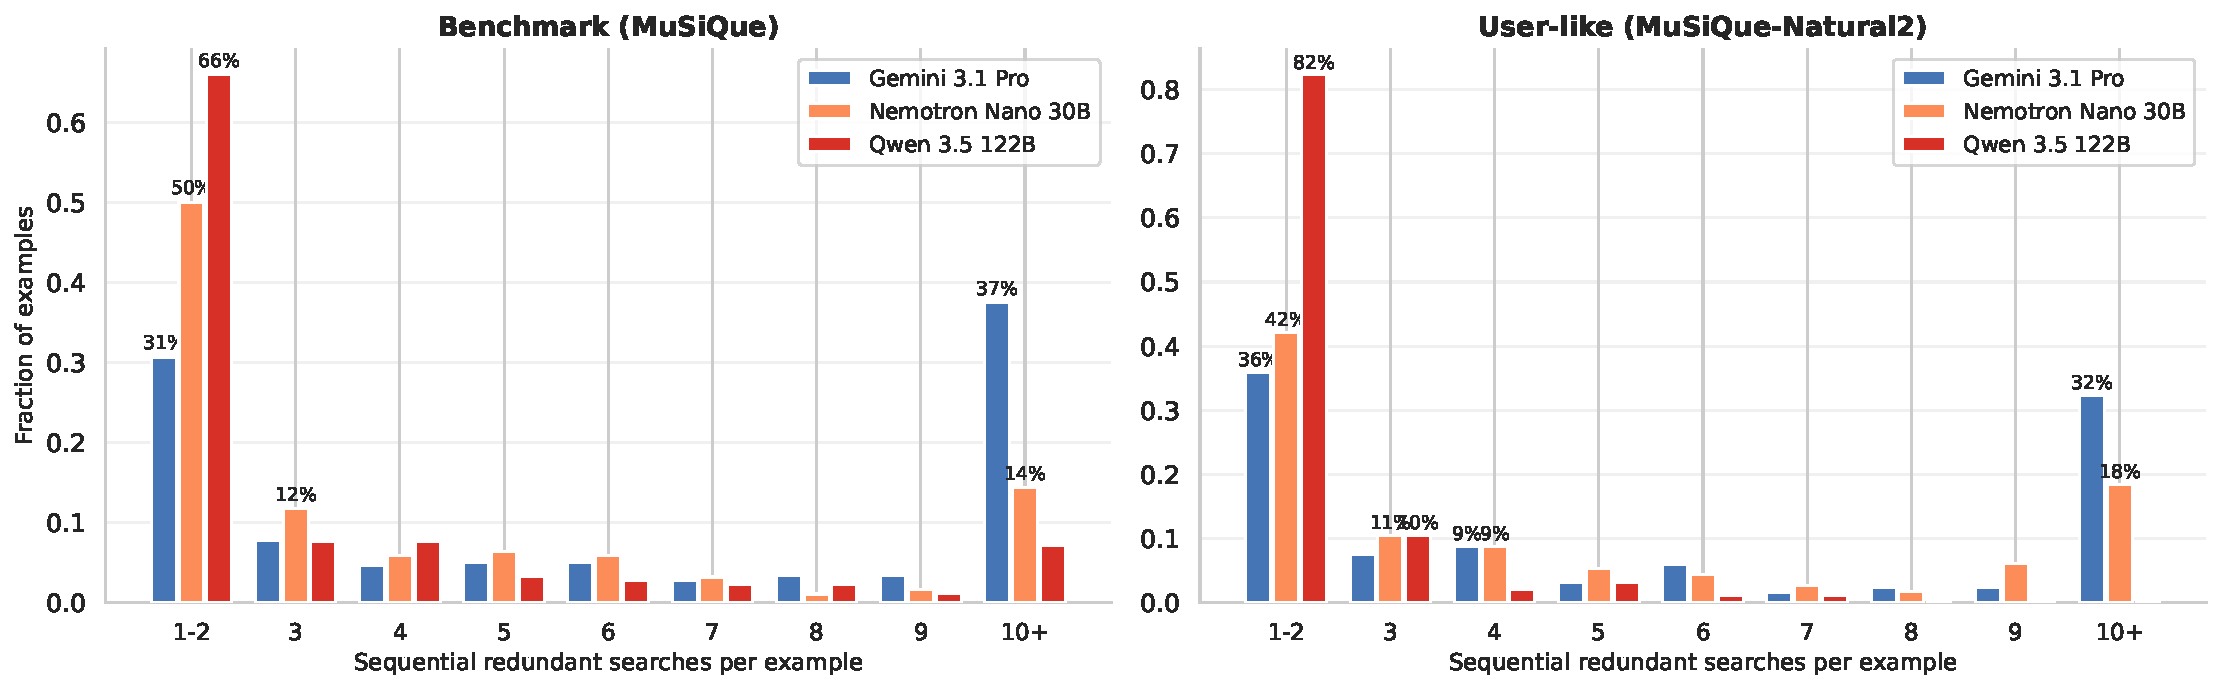
\includegraphics[width=\linewidth]{Figures/sequential_redundancy_distribution.pdf}
  \caption{Sequential redundancy distribution. The high redundancy in the benchmark condition stems from the under-utilization of previous search results that already contain the gold answer, leading to sequential redundant queries.}
  \label{fig:redundancy}
\end{figure}

\subsection{Search Efficiency and Pre-Search Commitment}\label{sec:efficiency}

Under benchmark phrasing, models exhibit significant sequential search inefficiency, where redundant queries account for 28\% of searches (Figure~\ref{fig:redundancy}). We view this sequential redundancy as evidence of models overfitting to the behavioral patterns of the benchmark; rather than learning an optimal information-seeking policy, models memorize the specific search trajectories expected by the training data, continuing to issue redundant follow-up queries simply because it matches the structural patterns they were overfitted on. However, this redundant behavior is highly reduced under natural phrasing in comparison. Unfortunately, under user-like phrasing, the overall search budget shrinks from the wrong cells: redundant searching falls \emph{together with} effective searching, moving agents from sequential redundancy to severe under-searching.

\begin{figure}[ht]
  \centering
  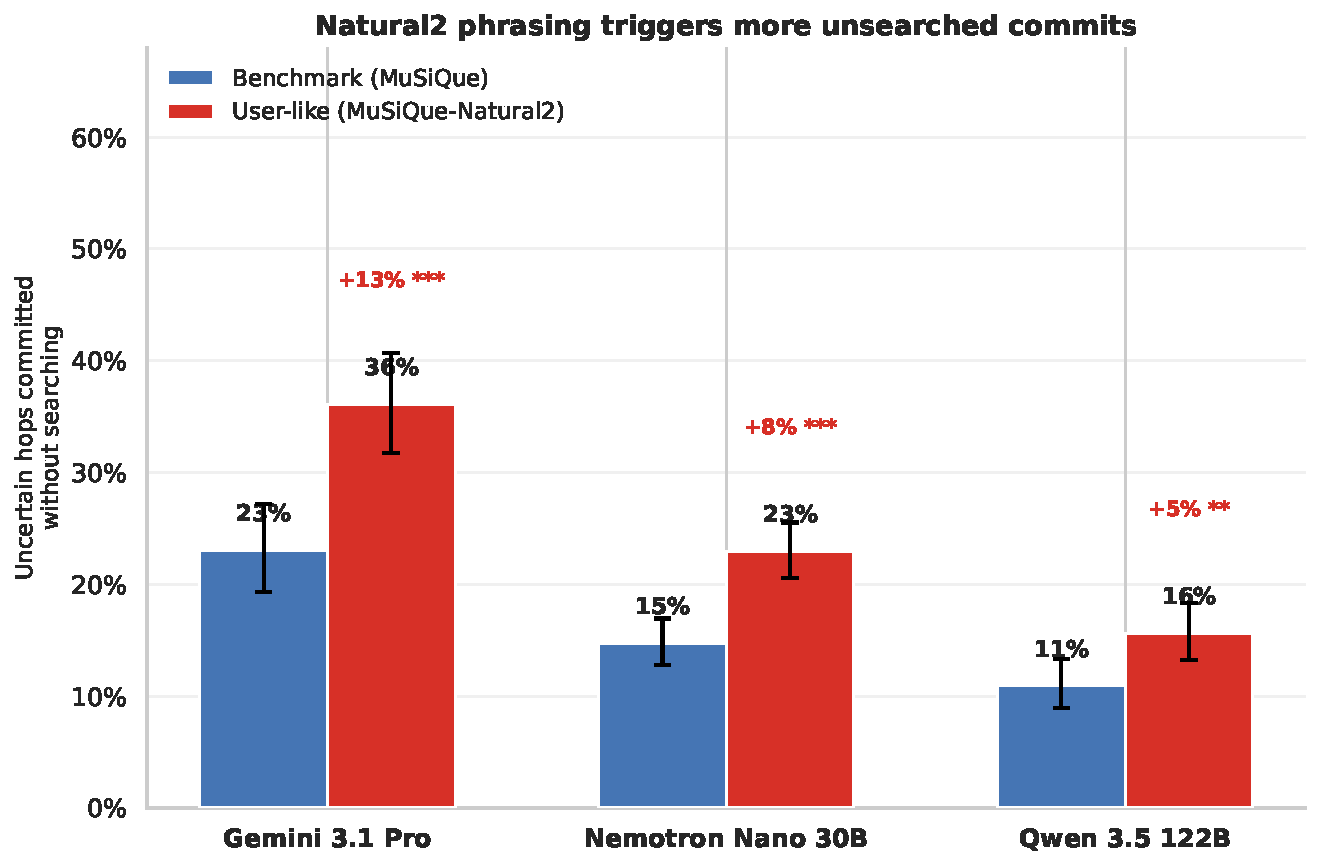
\includegraphics[width=0.8\linewidth]{Figures/fig1_early_commit_rate_benchmark_vs_nat2.pdf}
  \caption{Commitment-locus probe: The fraction of uncertain hops where the model prematurely commits to a parametric answer before issuing any search query, showing a sharp rise under Natural~2 phrasing compared to the benchmark.}
  \label{fig:commitment}
\end{figure}

Mechanistically, the failure stems from \emph{pre-search commitment}. To understand why the Missed cell grows under naturalistic phrasing, we introduce a \textbf{commitment-locus probe}. For every evaluated hop, an LLM judge identifies the first turn at which the agent commits to a specific answer for that hop's sub-question, and compares it to the first turn carrying a search query attributed to that same hop. 

As Figure~\ref{fig:commitment} shows, the fraction of uncertain hops on which the agent commits \emph{before} any such search rises sharply under user-like phrasing across all models. The agent is not merely delaying retrieval; it is actively substituting a parametric commitment for it on hops it had itself flagged as uncertain. Verbalized commitment to an answer moves upstream of retrieval as the phrasing becomes user-like. This reveals a critical framing-induced brittleness: the model internally recognizes a fact gap, but the user-like surface form triggers it to prematurely commit to a parametric guess, bypassing the search tool entirely.

\subsection{Intervention: Recovering Uncertainty-Aligned Search With a LoRA}\label{sec:intervention}

To demonstrate that pre-search commitment under user-like phrasing is a learnable alignment issue, we fine-tune \textbf{Nemotron Nano 30B} with a LoRA adapter on a curated supervised mix drawn from the model's \emph{own} on-policy rollouts. This mix teaches the model to search every uncertain hop, explicitly avoid searching certain ones, and leverages a phrasing augmentation that pairs formal questions with their natural paraphrases.

The intervention successfully recovers uncertainty-aligned search behavior. On Natural~1, the baseline Nemotron Nano 30B's \emph{Missed} cell drops significantly by 8.9 percentage points (20\% relative) and the \emph{Effective} cell rises by 8.9 percentage points (27\% relative) after SFT (Figure~\ref{fig:taxonomy}). This provides a direct, training-time demonstration that the benchmark-to-user behavioral gap is not a fixed capability deficit but a \emph{recoverable} signal. An explicit uncertainty-alignment objective, built from the model's own rollouts and surface-form augmentation, measurably restores the search-on-doubt behavior the model loses under user-like phrasing.

\section{Discussion}

Our investigation reveals a concerning vulnerability in modern agentic LLMs: the \emph{mis-generalization of tool-use behavior}. While these models achieve high performance on structured benchmarks, their ability to actively recognize knowledge gaps and deploy external tools severely degrades when confronted with naturalistic user queries. This breakdown highlights that current models often memorize the structural heuristics of their training data rather than internalizing a robust, generalized policy of ``searching when uncertain.''

A central takeaway from our analysis is the deceptive nature of end-to-end accuracy metrics. The fact that aggregate task accuracy remains stable despite a collapse in appropriate search behavior demonstrates that outcome-based evaluations often mask critical behavioral failures. Confounding factors such as parametric leakage and the regularizing effect of omitted noisy searches can artificially inflate performance metrics. This underscores the necessity of granular, trajectory-level diagnostics---such as our hop-level evaluation---to genuinely assess agentic alignment.

Mechanistically, the observed shift toward \emph{pre-search commitment} under user-like phrasing suggests a misalignment between a model's epistemic uncertainty and its action space. Even when models possess the internal capacity to detect their own knowledge gaps, unfamiliar surface forms trigger a premature reliance on parametric guessing over active information-seeking. In real-world deployments, particularly in domains susceptible to misinformation, agents that confidently hallucinate answers despite internal doubt pose a significant risk. 

However, our intervention with Nemotron Nano 30B provides an optimistic path forward. By successfully mitigating this brittleness via LoRA fine-tuning on on-policy rollouts, we demonstrate that uncertainty-aligned search behavior is a recoverable signal. It is not an insurmountable capability deficit but an alignment objective that can be explicitly targeted during post-training. 

Ultimately, distinguishing what a model knows from how it behaves is critical. We urge the community to expand the focus of agent evaluation and alignment beyond static end-task success, prioritizing robust behavioral policies that generalize safely to real-world, user-driven interactions.
\section{Limitations}

While our findings provide a novel perspective on the behavioral generalization of agentic LLMs, our study has several limitations.

First, our hop-level diagnostic protocol is heavily reliant on the MusiQue dataset. The rigorous evaluation of uncertainty alignment requires gold \emph{hop decompositions} to accurately map search queries and parametric answers to specific knowledge gaps. Consequently, the scope of our primary evaluation is constrained to datasets that provide these structured sub-hops, limiting the diversity of tasks we can probe.

Second, although our SFT intervention via LoRA successfully recovered the underlying uncertainty-aligned search signal, it also exhibited side effects. While it significantly reduced the number of missed searches on uncertain hops, we observed an overall increase in the total search rate, including a rise in parametrically redundant searches. This suggests that while models can learn to be less over-confident, balancing this alignment without inducing a generic ``over-searching'' bias remains a challenge.

Third, our methodology relies on automated LLM judges for critical pipeline steps: query paraphrasing, semantic equivalency verification (for Natural~2), and attributing search queries to specific hops. While we employed a conservative \emph{generate$\to$judge$\to$regenerate} validation loop to mitigate confounding factors, the inherent biases and occasional hallucination of LLM-as-a-judge paradigms introduce a degree of unavoidable noise into the evaluation.

Finally, our setup estimates epistemic uncertainty via semantic entropy, which requires sampling multiple generations per hop. This process is computationally intensive and largely impractical for real-time inference in deployed systems. Furthermore, our evaluation focuses on single-turn multi-hop queries; exploring how behavioral mis-generalizations compound over extended, multi-turn conversational workflows is an important direction for future work.

\section{Future Work}

Our findings open several avenues for future research into the behavioral alignment of agentic LLMs. First, the development of scalable, reference-free metrics to evaluate epistemic uncertainty without relying on computationally expensive semantic entropy sampling is crucial for real-time applications. Second, future studies should move beyond single-turn interactions to investigate how tool-use mis-generalization compounds over long-horizon, multi-turn conversations. Additionally, investigating reinforcement learning techniques that explicitly penalize parametrically redundant searches while rewarding searches on high-uncertainty hops could yield more robust and balanced policies than SFT alone. Finally, extending our hop-level diagnostic framework to broader domains, such as code generation, mathematical reasoning, and automated data analysis, will be vital to understanding the full extent of behavioral mis-generalization across different task distributions.
\bibliographystyle{plainnat}
\bibliography{bibliography}


\appendix
\section{Additional Search Calibration Plots}\label{app:calibration}

\begin{figure}[ht]
  \centering
  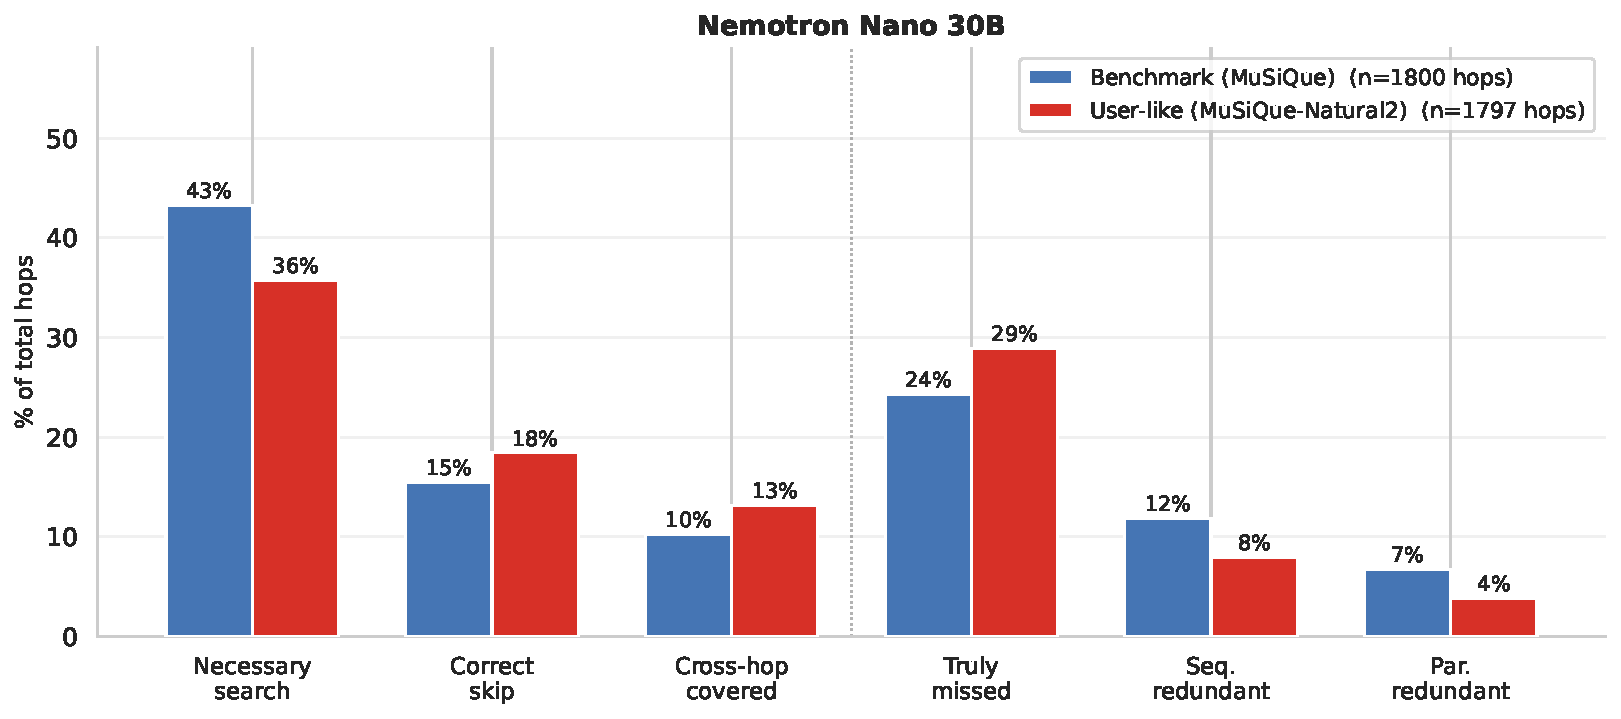
\includegraphics[width=0.8\linewidth]{Figures/search_calibration_extended_nemotron_3_nano_30b.pdf}
  \caption{Search calibration for Nemotron Nano 30B.}
\end{figure}

\begin{figure}[ht]
  \centering
  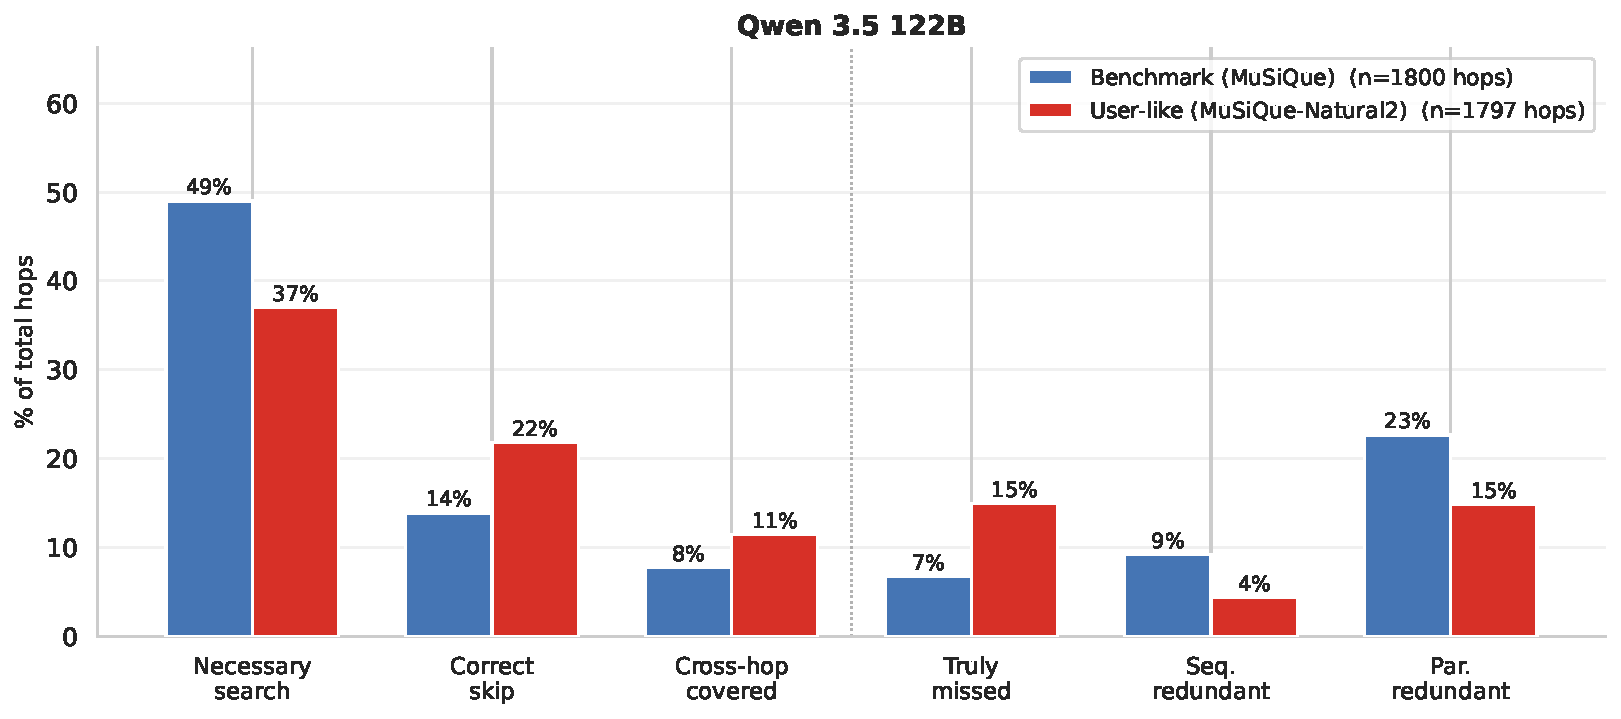
\includegraphics[width=0.8\linewidth]{Figures/search_calibration_extended_qwen3_5_122b.pdf}
  \caption{Search calibration for Qwen 3.5 122B.}
\end{figure}

\section{Knowledge Tiers of Missed Searches}\label{app:knowledge_tiers}

\begin{figure}[ht]
  \centering
  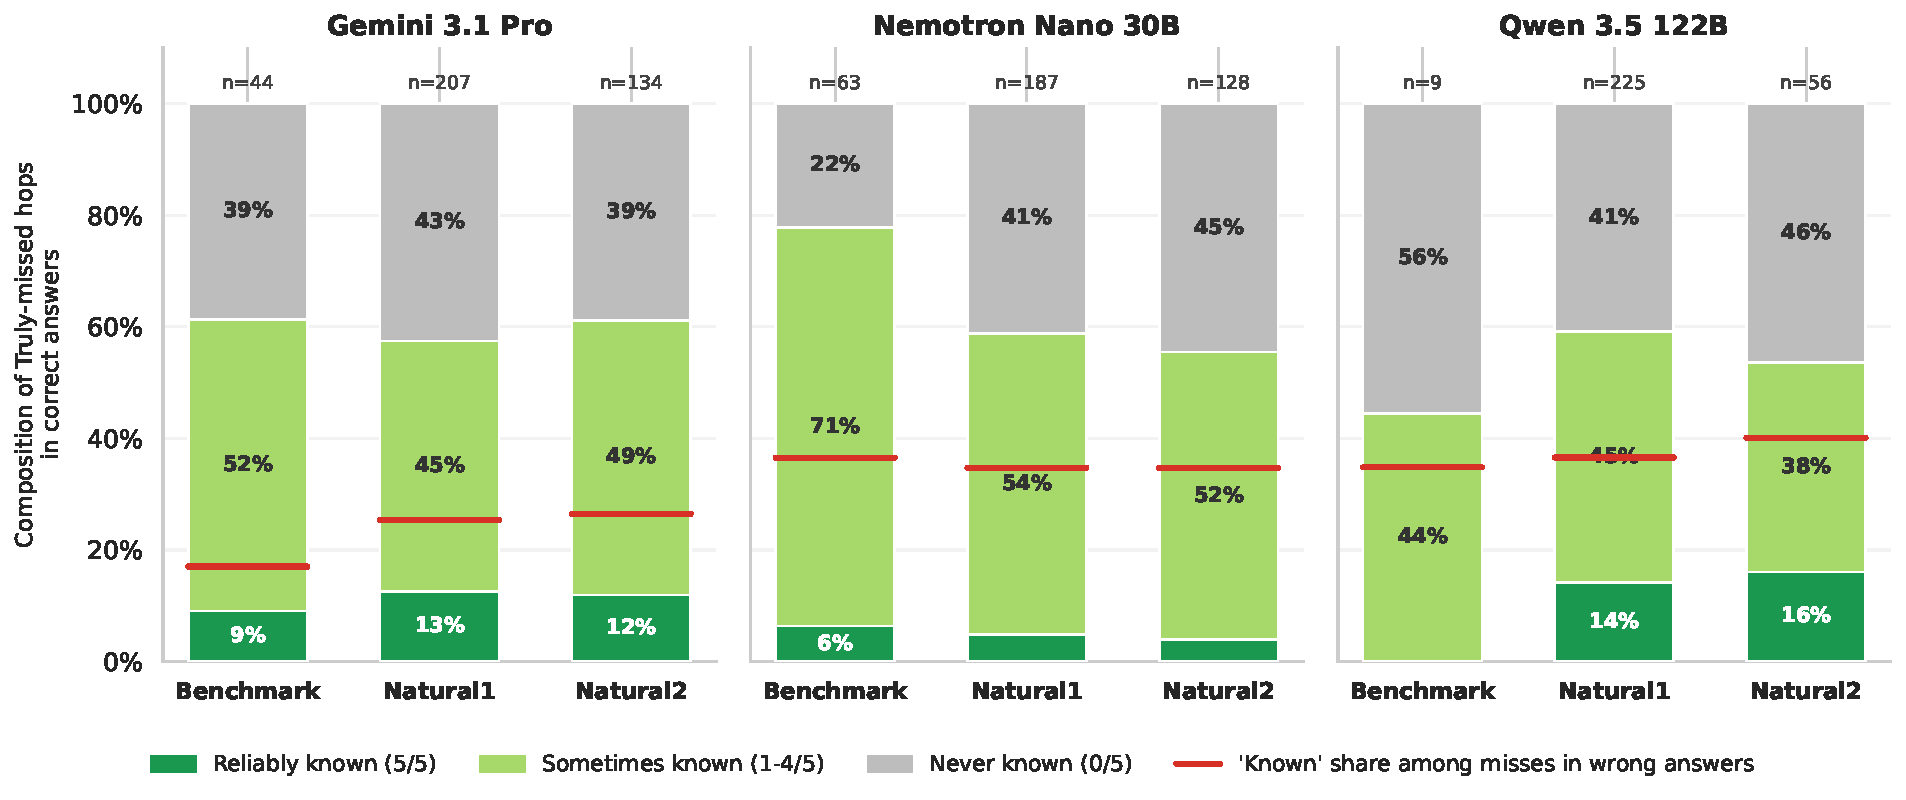
\includegraphics[width=0.8\linewidth]{Figures/missed_hop_knowledge_tiers.pdf}
  \caption{Missed hops distributed across knowledge tiers, illustrating the continuous spectrum of uncertainty.}
  \label{fig:knowledge_tiers}
\end{figure}

\end{document}